\section{Kinematic position angle analysis}
\label{sec:methods-I-kinemetry}

\subsection{Kinematic position angle analysis}
Kinematic position angle PA$_{k}$  analysis involves the determination of the orientation of the major axes of gas and stellar velocity fields. One application of the method is to distinguish disc dominated systems from those systems displaying a complex morphology. Discs generally have co-rotational velocity fields and well aligned position angles, while merged systems may contain distinct kinematic components, until the components coalesce dynamically. Merged systems can exhibit misaligned position angles of their gas and stellar velocity fields. The difference in the global position angles of the major axes of stellar and gas velocity field yields the quantity $\Delta$PA$_{k}$ (measured in degrees).

%TC:ignore
\red{\citet{2011MNRAS.414.2923K} investigated the relationships between the morphologies, kinemetric features and alignment between photometric and kinematic axes of early-type galaxies in the ATLAS$^{3D}$ project.}

\red{Kinematic position angle $\Delta$PA$_k$ analysis was employed in the study of galaxy interaction the Calor Alto CALIFA survey \citet{2015A&A...582A..21B} studied a sample of 103 interacting galaxies at various merger stages: close companions, systems with evidence of morphological interaction and coalesced merger remnants. Classification of these systems was performed by measuring the difference in kinematic position angles of the stellar and ionised gas velocity fields. A sample of 80 non-interacting galaxies was used as a control sample. Their findings revealed that 42\% of interacting galaxies have a misalignment of over 16\textdegree\ while this is evident in only 10\% of the control sample.}

\red{In a similarly motivated study \citet{2016A&A...591A..85B} examined the gas kinematics of nearby (ultra)luminous infrared galaxies ((U)LIRGs) at $z<0.1$. The objective was to analyse the kinematic properties of local (U)LIRGs and characterise their structures as those (U)LIRGs having disc structures (disc class), or displaying evidence of major merger activity (merger class). Their method employs optical integral field spectroscopy (IFS) data obtained at the VLT. H$\alpha$ emission is used as a gas velocity tracer. \citet{2016A&A...591A..85B} conclude that their results confirm that well-defined discs can be effectively distinguished from well-defined mergers but there is intermediate, indeterminate class.}
%TC:endignore

\subsection{Kinematic PA analysis method description}
\label{sec:kinemetry-analysis-method-description}
% \subsection{Quality screening}
Global kinematic velocity position angles (PA$_{k}$) for the PSB and control galaxy samples were determined using the \texttt{fit\_kinemetry\_pa} IDL routine as described in appendix C of \cite{2006MNRAS.366..787K}. The code returns the angle of the line bisecting the greatest change in a stellar or gas velocity field between the receding and approaching sides. The \texttt{fit\_kinemetry\_pa} IDL code and a Python 3 package \texttt{PaFit} are available via Michele Cappellari's website\footnote{\href{http://www-astro.physics.ox.ac.uk/~mxc/software/\#pafit}{http://www-astro.physics.ox.ac.uk/~mxc/software/\#pafit}}. We downloaded the \texttt{PaFit} package and successfully tested this code fitting kinematic position angles to the model velocity fields provided. 


\cite{2019MNRAS.483..172D} performed a kinematic position angle analysis on over 8,000 galaxies from the MaNGA Product Launch MPL-8 internal data release. In order to obtain a clean sample of well defined global PAs they visually classified the stellar and H$\alpha$ gas velocity fields of all galaxies in their sample into 3 categories (Chris Duckworth, 2019, personal communication), and set flags in their dataset as follows:

\begin{itemize}
    \item {Flag 1}  Dominant coherent rotation and well defined PA
    \item {Flag 2}  Dominant coherent rotation but with complex motions or highly inclined velocity fields 
    \item {Flag 3}  Do not use
\end{itemize}

The resulting MPL-8 screened dataset of galaxies with reliable global PAs (flagged as [1] or [2]) from \cite{2019MNRAS.483..172D} was matched with the PSB galaxies in the sample of Chen et al. (2019, submitted.) to obtain a subset of PSBs with good velocity field analysis analysis flags.

Examples of misaligned stellar and gas velocity fields for a CPSB and an RPSB is shown in Figure \ref{fig:CPSB-8313-6101-PA}. In classical kinematic position angle analysis it is considered significant if the gas and stellar velocity field offset position angle $\Delta$PA$_{k}$ is greater than 30\textdegree. This can be an indication of past disruption of the galaxy.

\begin{figure*}
    \centering
    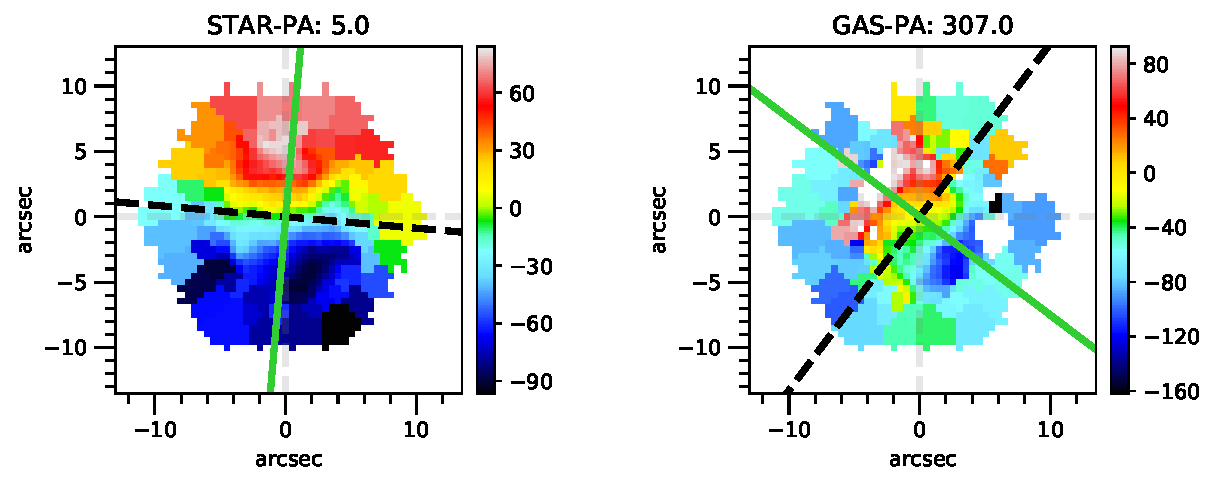
\includegraphics[width=0.8\textwidth]{images/PAplots/PAplotsCPSB/8313-6101-PA.pdf}
    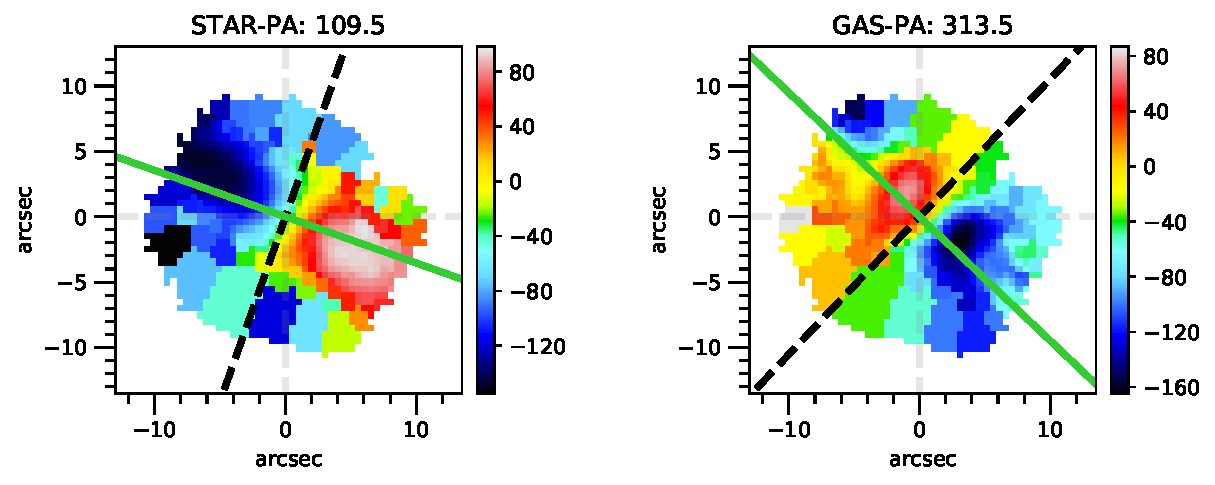
\includegraphics[width=0.8\textwidth]{images/PAplots/PAplotsRPSB/8323-6103-PA.pdf}
    \caption[Examples of PSBs showing significant kinematic PA misalignment $\Delta$PA$_{k}$: CPSB 8313-6101 and RPSB 8323-6103.]{Illustration of velocity field maps for PSBs with fitted kinematic position angles (PA$_{k}$) showing considerable misalignment. The stellar velocity fields (left) and gas velocity fields (right) are shown for CPSB 8313-6101 (top), and RPSB 8323-6103 (bottom). The position angles of the velocity field (gas or stars) are displayed as green solid lines, while the black dashed lines denotes the bisector of the velocity fields between the receding (red) and approaching (blue) sides. The velocity colour scale is \kms. Credit for data analysis and plots: Chris Duckworth.}
    \label{fig:CPSB-8313-6101-PA}
\end{figure*}


